\chapter{ScatterPlot View}
\label{sec:scatter_view}

A ScatterPlot View displays the distribution of two numerical variables as points. When started, it presents itself in the following manner.

\begin{figure}[H]
    \centering
    \hspace*{-2.5cm}
    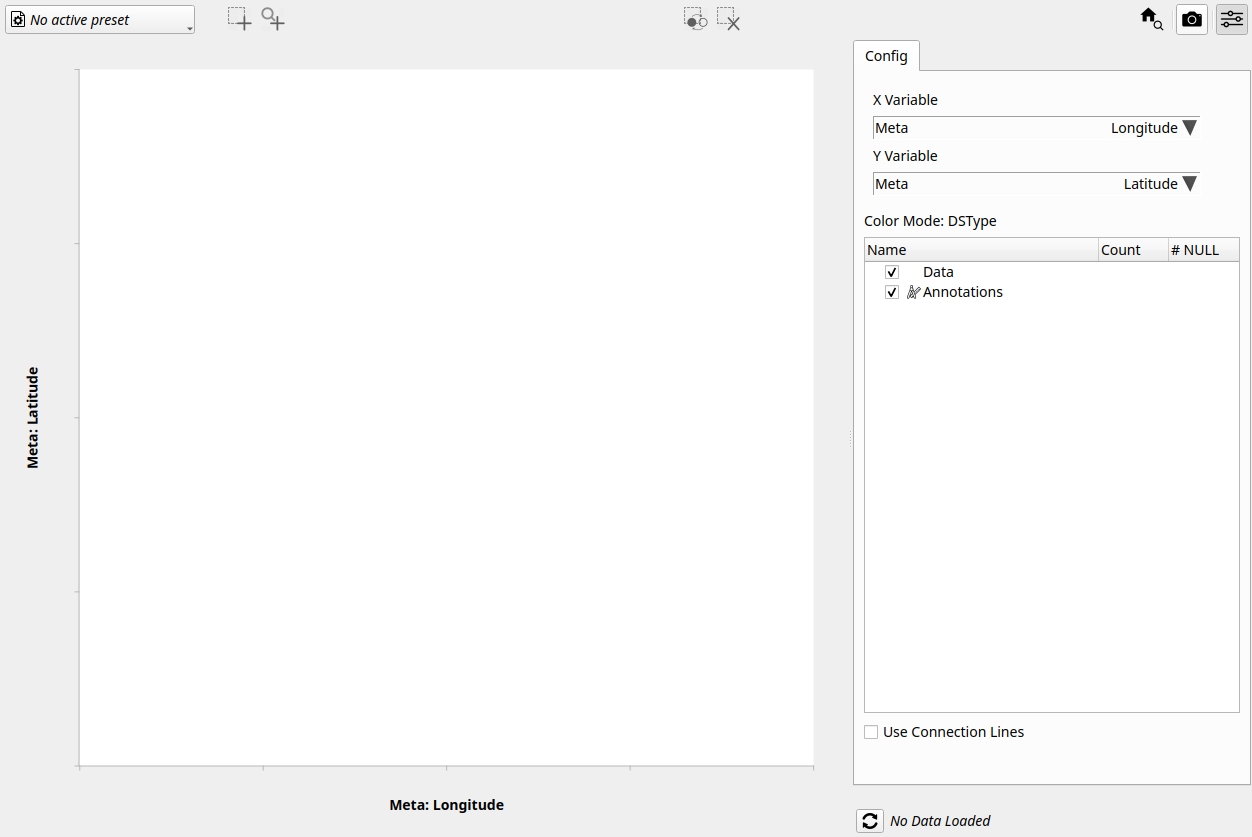
\includegraphics[width=19cm,frame]{figures/scatter_start.png}
  \caption{ScatterPlot View startup}
\end{figure}

\section{Layout}

On the left side resides the plot area in which the data is visualized (if data has been loaded). The tool bar at the top shows the currently selected tool and the available actions.\\

On the right side resides the configuration area, which allows configuring what data is loaded and how it is displayed. The 'Reload' button on the bottom can be used to trigger a reload of the view's data.\\

Both areas can be resized and hidden if desired.

\section{Data Loading}

To load the data the mechanism described in section \nameref{sec:ui_overview} or the 'Reload' button can be used. To filter the dataset, the mechanism described in section \nameref{sec:filters} can be used. \\

\begin{figure}[H]
    \centering
    \hspace*{-2.5cm}
    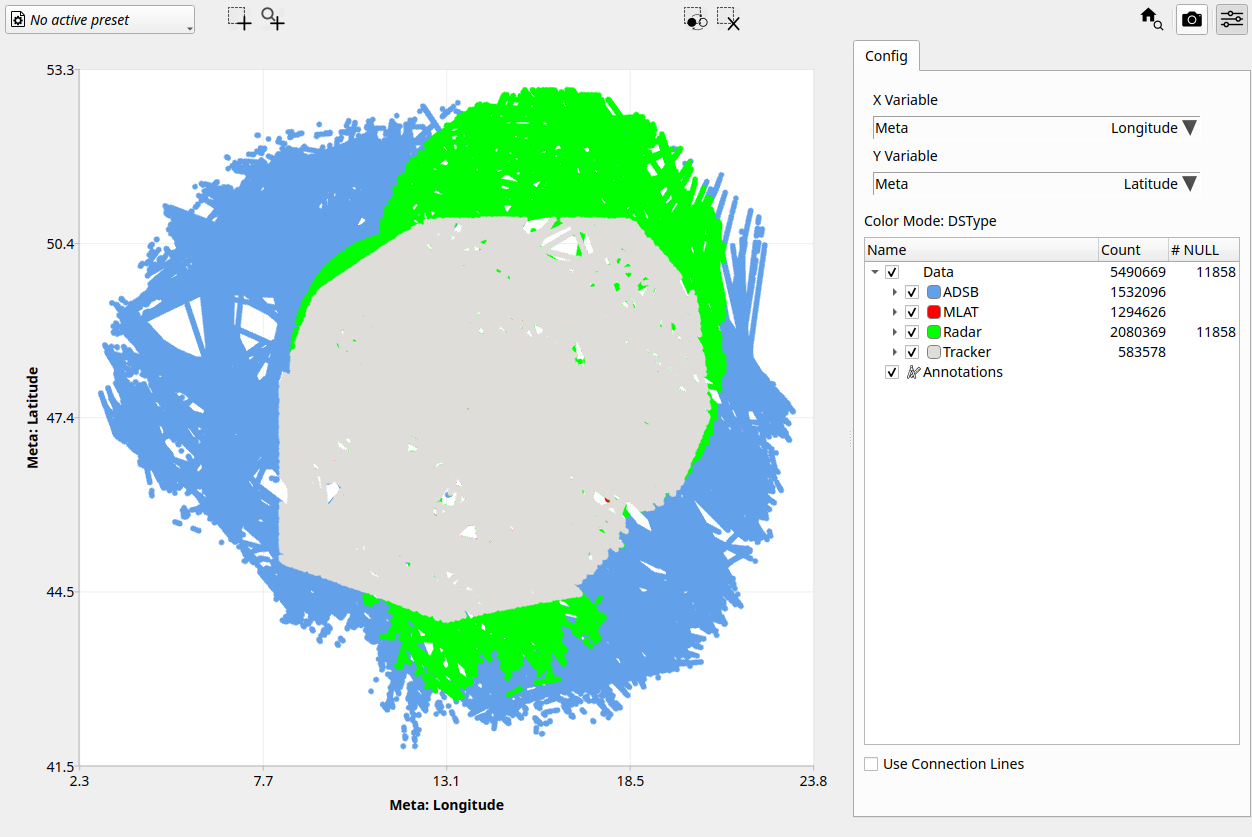
\includegraphics[width=19cm,frame]{figures/scatter_loaded.png}
  \caption{ScatterPlot View after loading data}
\end{figure}

The values of the selected variables are used for positioning on the x-axis and y-axis. For each value pair a data point is generated. 
In the current example the WGS-84 meta-variables 'Longitude' and 'Latitude' are used, showing a similar view as the Geographic View. \\

Data points are colored according to the global Color Mode (see \nameref{sec:color_mode}); the legend reflects the chosen coloring level (DSType, DBContent, Data Source, or Data Source + Line). \\

Colors come from the active Data Context's palette, so the same Data Source / DSType keeps the same color across reloads and across all Views. Series visibility also persists across reloads; this is driven entirely by the shared mechanism, no per-view persistence control exists.

\section{Usage}

\subsection{Toolbar}

The first buttons can be used to switch between the available tools (shortcut refers to keyboard shortcut).

Note that an active tool can always be ended by pressing the 'Escape' key. 

\begin{table}[H]
  \center
  \begin{tabular}{ | l | l | l | l |}
    \hline
    \textbf{Icon} & \textbf{Shortcut} & \textbf{Text} &  \textbf{Description} \\ \hline
    \includegraphics[width=0.5cm,frame]{../../data/icons/select_action.png} & S & Select & Allows data selection \& de-selection \\ \hline
    \includegraphics[width=0.5cm,frame]{../../data/icons/zoom_select_action.png} & R & Zoom to Rectangle & Allows zooming to the selected rectangle \\ \hline
    
  \end{tabular}
  \caption{Toolbar: Available tools}
\end{table}

The others provide general actions by which the view can be modified.

\begin{table}[H]
  \center
  \begin{tabular}{ | l | l | l | l |}
    \hline
    \textbf{Icon} & \textbf{Shortcut} &\textbf{Text} &  \textbf{Description} \\ \hline
    \includegraphics[width=0.5cm,frame]{../../data/icons/select_invert.png} & & Invert Selection & Selects all de-selected \& vice versa \\ \hline
    \includegraphics[width=0.5cm,frame]{../../data/icons/select_delete.png} & & Delete Selection & De-selects all target reports \\ \hline
    \includegraphics[width=0.5cm,frame]{../../data/icons/zoom_home.png} & Space & Zoom to Home & Pans/zooms to show all existing data \\ \hline
  \end{tabular}
  \caption{Toolbar: Available actions}
\end{table} 

\subsection{Config Tab}

The selection controls on the top define which data variables are used to generate data points for the x/y-axis.
Such a variable can be any numerical variable. A reload operation might be required for the selection to take effect. \\

The Config Tab includes the shared Layers Tree (see \nameref{sec:layers_tree}), which controls per-DBContent / per-Data-Source / per-line visibility for the scatter data items. The dedicated per-view annotation tab that existed in earlier releases has been removed; plottable scatter annotations of active View Points are now exposed under the 'Annotations' group of the Layers Tree. When multiple scatter annotations are present, the 'Plot' and (if available) 'Plot Group' combo boxes are used to choose between them. \\

Scatter data items can be drawn with their data points connected by lines by checking the 'Use Connection Lines' box.
\textbf{Note} that on a reload, if the total number of drawn data points exceeds 100000, connections lines will be deactivated automatically
in order to prevent performance issues. After the reload the connection lines can be reactivated manually by the user if desired.

\subsection{Scatterplot}

\subsubsection{Selection Tool}

If the 'Select' tool is active, data can be selected. Using the left mouse-button a red selection rectangle can be spanned across all data points that should be selected.

\begin{figure}[H]
    \centering
    \hspace*{-2.5cm}
    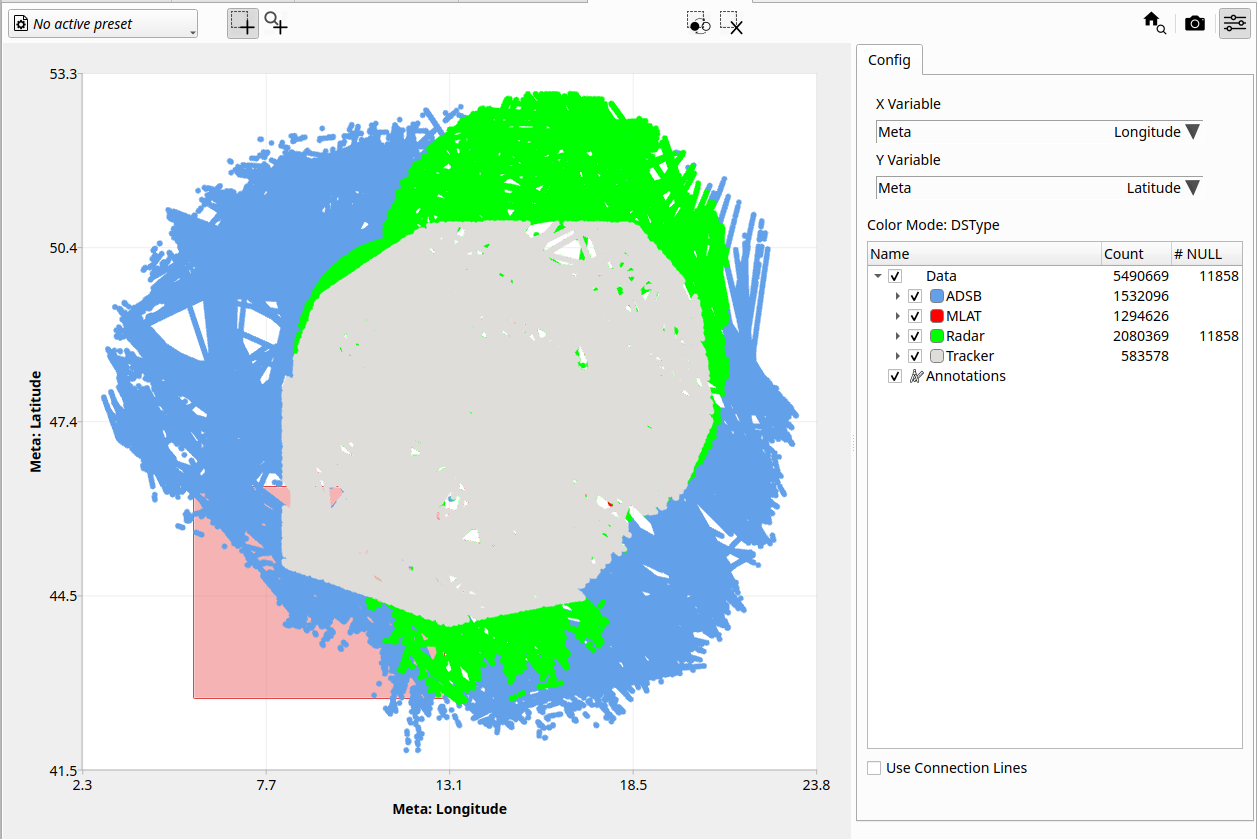
\includegraphics[width=19cm,frame]{figures/scatter_select.png}
  \caption{ScatterPlot View data selection}
\end{figure}

The selected data is then presented in an extra 'Selected' item in the scatter data list.

\begin{figure}[H]
    \centering
    \hspace*{-2.5cm}
    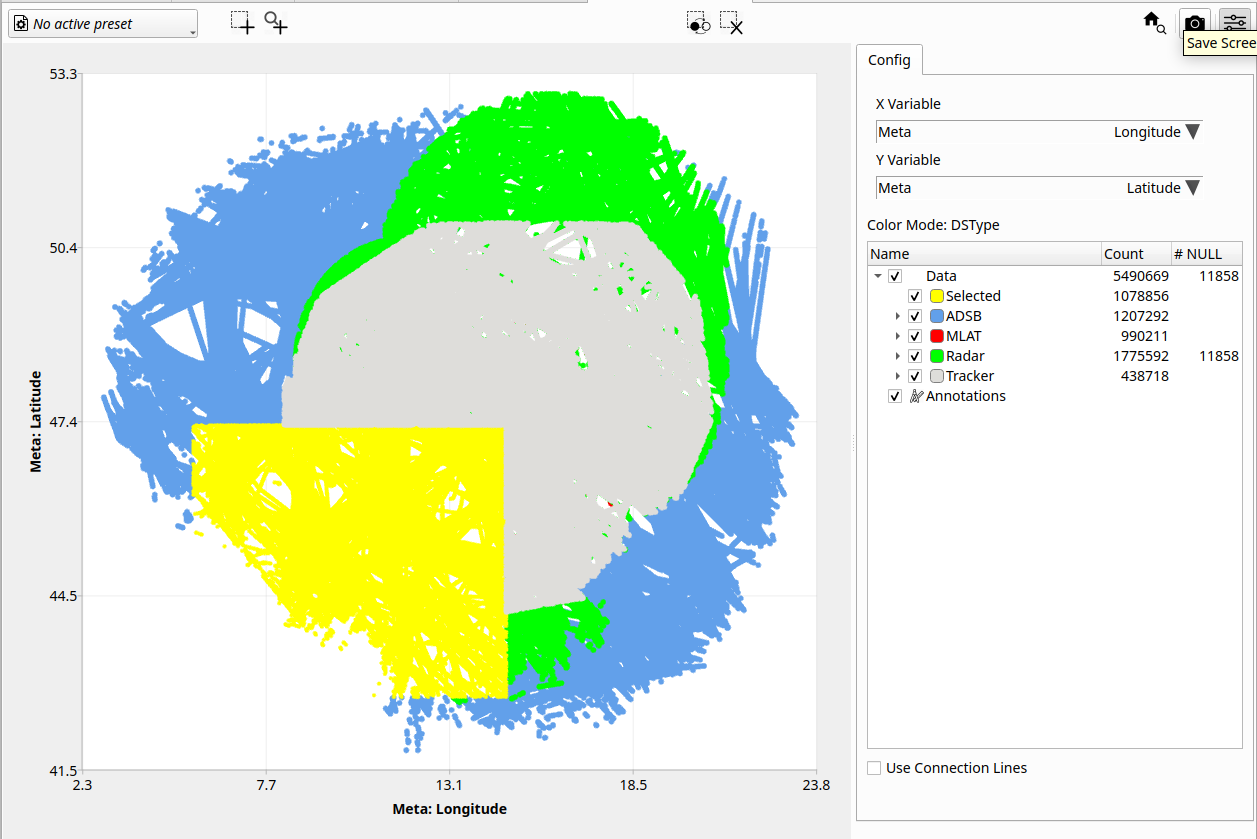
\includegraphics[width=19cm,frame]{figures/scatter_selected.png}
  \caption{ScatterPlot View data selected}
\end{figure}

This enables selection of parts of the data based on the presented variables, allowing deeper analysis e.g. of dubious data. \\

The 'Invert Selection' \includegraphics[width=0.5cm,frame]{../../data/icons/select_invert.png} or 'Delete Selection' \includegraphics[width=0.5cm,frame]{../../data/icons/select_delete.png} actions 
allow for easier selection of the wanted target reports. \\

By pressing the 'Control' key while selecting, the newly selected data is added to any previous selection. This can be used to select data incrementally, making more complex selections possible.

\subsubsection{Zoom to Rectangle Tool}

Using the 'Zoom to Rectangle' tool, the left mouse-button can be used to select a rectangular region, to which a zoom operation is performed. \\

\subsubsection{General Zoom}

The mouse wheel can be used to zoom in or out of the presented data, the 'Space' key can be used to reset to the default zoom level (equivalent to \includegraphics[width=0.5cm,frame]{../../data/icons/zoom_home.png}).
